\documentclass[a4paper,runningheads]{llncs}
\usepackage[T1]{fontenc}
\usepackage{graphicx}
\usepackage{booktabs}
\usepackage{amsmath,amssymb}
\usepackage{microtype}
\usepackage{url}
\usepackage{xurl}
\AtBeginDocument{\renewcommand{\doi}[1]{\url{https://doi.org/#1}}}
\usepackage{cite}
\usepackage{xcolor}

\InputIfFileExists{generated/macros.tex}{}{}
\InputIfFileExists{generated/macros_review.tex}{}{}
% Fallbacks shown only if a result file is missing.
\providecommand{\PermMaxCarf}{??}\providecommand{\NPerm}{??}\providecommand{\PermPCarf}{??}

\newcommand{\logit}{\operatorname{logit}}
\newcommand{\clip}{\operatorname{clip}}

\pdfinfoomitdate=1
\pdftrailerid{}
\pdfsuppressptexinfo=-1
\begin{document}
\title{CARF: Bounded Anchored Fusion for Multimodal Prediction with Unreliable Modalities}
\titlerunning{CARF: Bounded Anchored Fusion}
\author{Sachin Kumar\inst{1}\orcidID{0009-0007-2893-0655} \and
Subhankar Mishra\inst{1}\orcidID{0000-0002-9910-7291}}

\institute{School of Computer Sciences, National Institute of Science Education and Research (NISER), Bhubaneswar, India\\
\email{smishra@niser.ac.in}}
\maketitle

\begin{abstract}
In clinical prediction, some inputs are missing or silently wrong, e.g., after a specimen swap. We propose Clinical-Anchored Residual Fusion (CARF), which keeps an always-available clinical model's logit as an anchor and lets each optional modality move it only within a log-odds budget. An \emph{anchor-verification gate} scales each optional contribution by the posterior probability that the sample belongs to the patient, estimated from auxiliary hormone-receptor and HER2 heads. The convex objective and exact mask handling keep exact fallback to the anchor and a per-patient bound on prediction change. For pathological complete response, we combine a treatment-aware anchor with expression, MRI, and a proteomic modality available for part of the cohort. On \NDev{} I-SPY2 patients, CARF's AUROC (\IntCarfTwo{}) is statistically indistinguishable from unconstrained fusion. On external I-SPY1, the bound matters: CARF's worst-case AUROC over modality failures (\ExtWorstCarfTwo{}) beats every baseline except a gated robust offset model, and no prediction moves more than \MaxDispCarfTwo{} logits. Its advantage grows when two optional modalities fail together (\ComboSwapSwapCarf{} vs.\ \ComboSwapSwapRobustOffsetLr{}), but it reverses if the clinical anchor is corrupted, where CARF loses more than stacking (\AnchorBothTwoZeroCarf{} vs.\ \AnchorBothTwoZeroStack{} at 20\% HR/HER2 errors).\keywords{Multimodal learning \and Missing modalities \and Robust fusion \and Sample verification \and Bounded influence}
\end{abstract}

%======================================================================
\section{Introduction}

Multimodal learning combines heterogeneous sources of information about the same individual \cite{baltrusaitis2019}. In clinical applications, some inputs are recorded for every patient, while others are optional, site-dependent, or of unknown quality. A fusion model can depend on an optional modality more than is safe when it is absent or wrong. Stacking \cite{wolpert1992} and learned gates may weight an expert that is accurate on training data heavily, and confidence does not remove this risk: after a sample swap, the output is plausible and confident but uninformative.

We study pathological complete response (pCR), i.e., no invasive cancer at surgery after neoadjuvant chemotherapy, in the I-SPY1 \cite{esserman2012} and I-SPY2 \cite{wolf2022ispy} breast cancer trials. Clinical variables (hormone-receptor (HR) and HER2 status, planned regimen) are available for all patients, whereas gene expression, dynamic contrast-enhanced MRI, and reverse-phase protein arrays (RPPA) are optional. RPPA was measured for \NRppa{} of the \NDev{} I-SPY2 patients and for none of the I-SPY1 patients.

We propose Clinical-Anchored Residual Fusion (CARF), in which optional modalities adjust the always-available clinical prediction only within a bounded budget. Its components are: (i) a mask-aware fusion rule with exact fallback to the anchor; (ii) an \emph{anchor-verification gate} scaling each optional residual by the posterior probability its sample matches the clinical HR/HER2 record; (iii) a convex objective over missingness and sample swaps, with the budget chosen by inner cross-validation; and (iv) an evaluation giving every baseline the same gate, testing mix-ups, simultaneous failures, anchor corruption, recalibration, decision-curve analysis, and confidence intervals.
%======================================================================
\section{Related Work}

ModDrop \cite{neverova2015} and related schemes \cite{ma2021smil} make fusion models tolerate absent modalities via dropout training, without limiting how much a corrupted modality can change a prediction. Several approaches weight experts by estimated quality: QA-MoE \cite{sun2026} separates quality estimation from routing for noisy, missing-modality clinical prediction, QMF \cite{zhang2023qmf} gives generalization guarantees for uncertainty-weighted late fusion, and Moon et al.~\cite{moon2026} question whether such scores change downstream decisions, since they come from the modality itself and cannot detect a confident expert applied to a swapped sample. Offset logistic regression is the standard way to update a clinical model with new predictors \cite{janssen2008}, and UCMR-Net \cite{tang2026} adds adaptive residuals to a text anchor without bounding the total correction. Our fitting objective is related to distributionally robust optimization \cite{sagawa2020}, with environments that are availability patterns and failures of the optional experts. CARF instead bounds the correction by construction and verifies each optional sample against variables recorded for every patient.

%======================================================================
\section{Approach}

Consider a binary outcome $y$ and experts that are each trained on one modality. The anchor expert outputs a probability $p_C$ for every patient; the optional experts $j=1,\dots,K$ output probabilities $p_j$ with availability indicators $m_j\in\{0,1\}$. Let $a=\logit(p_C)$ be the anchor logit and $d_j=\logit(p_j)-a$. We seek a fusion rule that (i) returns $a$ exactly when all optional inputs are absent, (ii) keeps the fused logit within a known distance of $a$, (iii) reduces the contribution of an optional sample that is inconsistent with the patient's record, and (iv) is fitted with a procedure that accounts for missing and failing optional inputs.

\subsection{Anchored residual fusion}

For each optional expert, CARF clips the logit difference to $[-B,B]$, i.e., $r_j=\clip(d_j,-B,B)$, and scales it by three context functions with values in $[0,1]$: $h_{j0}=1$, $h_{j1}=e^{-|d_j|}$, which reduces the correction when the expert strongly disagrees with the anchor, and $h_{j2}=1-H(p_j)/\log2$, with the binary entropy $H$, which allows a different correction for confident experts. With the verification gate $g_j\in[0,1]$ defined below, the fused logit is
\begin{equation}
 z_\theta = a + \sum_{j=1}^{K}\sum_{k=0}^{2}\theta_{jk}\, m_j\, g_j\, h_{jk}\, r_j,
 \qquad \theta_{jk}\ge 0,\qquad \sum_{j,k}\theta_{jk}\le 1 .
 \label{eq:carf}
\end{equation}
A missing modality contributes zero, so that absence is represented by the mask and never by an imputed probability; since the coefficients are nonnegative, CARF can reduce the influence of an optional expert but cannot reverse its direction (Fig.~\ref{fig:architecture}).

\begin{figure}[t]
\centering
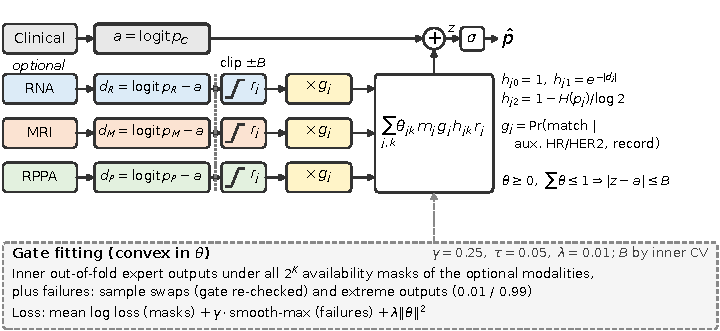
\includegraphics[width=0.78\linewidth]{figures/fig_architecture.pdf}
\caption{CARF with a clinical anchor (C) and optional RNA (R), MRI (M), and RPPA (P) experts. Each optional expert contributes a clipped residual $r_j$ relative to the anchor logit $a$, multiplied by its verification gate $g_j$, its mask $m_j$, and context functions $h_{jk}$, and weighted by $\theta\ge0$ with $\sum\theta\le1$. Auxiliary heads predict HR/HER2 from each optional modality; $g_j$ = posterior probability that the sample matches the clinical record.}
\label{fig:architecture}
\end{figure}

\paragraph{Anchor-verification gate.} The anchor contains variables that are also reflected in the optional modalities: HR and HER2 status are recorded clinically and are strongly associated with the expression of the corresponding genes and proteins. For each optional modality $j$, we train auxiliary logistic heads $q_{jt}$ that predict the anchor variables $t\in\{\mathrm{HR},\mathrm{HER2}\}$ from the modality, without the outcome. For a patient with recorded values $c_t$, let $\ell_j=\prod_t q_{jt}^{c_t}(1-q_{jt})^{1-c_t}$ be the likelihood of the record under the patient's own sample, and let $\bar\ell_j$ be the same quantity averaged over the samples of the training patients, i.e., the likelihood if the sample came from a random other patient. The gate is the posterior probability of a match,
\begin{equation}
 g_j = \Pr(\text{match}\mid q_j, c) = \frac{\pi\,\ell_j}{\pi\,\ell_j+(1-\pi)\,\bar\ell_j},
 \label{eq:gate}
\end{equation}
with a prior $\pi$ that mix-ups are rare ($\pi=0.95$). The gate needs no labels beyond the anchor and is computed per patient at prediction time. If a modality carries no information about the anchor variables, then $\ell_j\approx\bar\ell_j$ and $g_j\approx\pi$ for every patient, so an uninformative check leaves the fusion unchanged up to a constant that the coefficients $\theta$ absorb. Unrecorded anchor variables are skipped.

\subsection{Properties}
\label{sec:properties}

Let $b_j=B\sum_k\theta_{jk}$ be the budget of modality $j$ and $b=\sum_jb_j\le B$ the total budget. Since every summand of Eq.~\eqref{eq:carf} satisfies $|m_jg_jh_{jk}r_j|\le B$ and depends only on the anchor and on modality $j$, three properties hold for any values of the optional inputs. \emph{Fallback:} if all $m_j=0$, then $z_\theta=a$. \emph{Bounded displacement:} $|z_\theta-a|\le b$, and hence $|\hat p-p_C|\le b/4$. Replacing, removing, or swapping the sample of modality $j$ alone changes $z_\theta$ by at most $2b_j$. \emph{Ranking certificate:} two patients whose anchor logits differ by more than $2b$ keep their anchor ordering for any optional inputs. All statements also hold with the sharper budget $b^*_j=B\theta_{j0}+\kappa\theta_{j1}+B\theta_{j2}$, with $\kappa=\max_{t\le B}te^{-t}$. The verification gate can only shrink the residuals, so it does not weaken any bound.

\subsection{Convex robust gate fitting}

The gate coefficients $\theta$ are fitted on out-of-fold expert and auxiliary predictions obtained by five-fold cross-fitting within the training set. Let $L_e(\theta)$ be the mean logistic loss of $z_\theta$ in environment $e$. The set $\mathcal M$ contains all $2^K$ availability patterns of the optional modalities, and the set $\mathcal F$ contains failure environments: for each optional modality, four sample swaps, in which the modality's outputs are permuted among the patients who have it and the verification gate is recomputed against the receiving patient's record, and two extreme outputs ($0.01$ and $0.99$). We minimize
\begin{equation}
 \min_{\theta\ge0,\ \mathbf 1^\top\theta\le1}\;
 \frac1{|\mathcal M|}\sum_{e\in\mathcal M}L_e(\theta)
 +\gamma\,\tau\log\Big(\frac1{|\mathcal F|}\sum_{e\in\mathcal F}e^{L_e(\theta)/\tau}\Big)
 +\frac\lambda2\|\theta\|_2^2 .
 \label{eq:objective}
\end{equation}
The second term is a smoothed maximum over failures; since $z_\theta$ is linear in $\theta$ for fixed outputs, each $L_e$ is convex and the problem strictly convex over a polytope for $\lambda>0$, solved via sequential least-squares programming. We fix $\gamma=0.25$, $\tau=0.05$, $\lambda=0.01$, and choose $B\in\{1,1.5,2,3\}$ by inner five-fold cross-validation of the held-out objective (no penalty); no hyperparameter is chosen on an evaluation cohort.

%======================================================================
\section{Experiments}

\subsection{Experimental setup}

\paragraph{Data.} Development uses \NDev{} I-SPY2 patients (\NDevPos{} with pCR). The external cohort is \NExt{} I-SPY1 patients (\NExtPos{} with pCR) with expression and MRI; 87 more have a naturally missing modality, and GSE25066 \cite{hatzis2011} (409 patients, I-SPY1 samples excluded) is independent. Expression covers the \NGenes{} genes shared by both platforms; MRI features come from tumor masks in the BreastDCEDL release \cite{fridman2026} of TCIA \cite{tciaispy1,tciaispy2}; RPPA (\NRppaFeat{} proteins \cite{wolf2022ispy}) is missing for 25\% of development patients and all external patients (full preprocessing in the supplement).

\paragraph{Experts.} The anchor is \emph{treatment-aware}: besides age, HR, and HER2 status, it includes four planned-therapy indicators (anti-HER2 antibody, immunotherapy, platinum, HER2 kinase inhibitor), known before treatment; in I-SPY1 only trastuzumab is used. Each expert is a class-balanced logistic regression with fixed hyperparameters on the seven anchor variables, 250 ANOVA-selected genes, \NMriFeat{} MRI features, or RPPA features, fit on patients who have them (full hyperparameters in the supplement); auxiliary heads use unweighted logistic regressions on the same inputs. All preprocessing is fitted within each training partition.

\paragraph{Protocol.} Internal evaluation uses five repeats of five-fold cross-validation on I-SPY2 with inner cross-fitting; external models use all of I-SPY2. I-SPY1 labels never fit models, but external results informed exploratory RNA screening, so I-SPY1 is not untouched.

\paragraph{Baselines.} Fusion models share the same expert outputs: the mean; stacking \cite{wolpert1992}; mask-stacking (stacking with availability indicators, trained on all patterns); offset logistic regression using the anchor logit as offset \cite{janssen2008}, plus a robust-objective version; and a ModDrop-style MLP \cite{neverova2015} on probabilities and indicators, with architecture chosen by inner cross-validation. To separate gate from bound, every baseline is also fitted to \emph{gated} experts, $\logit\tilde p_j=a+g_j(\logit p_j-a)$, using the gate of Eq.~\eqref{eq:gate}.

\paragraph{Metrics and stress tests.} Models are frozen before failures are simulated. Each optional modality is removed (\emph{missing}) or swapped with another patient's sample (\emph{swap}; 5 realizations per internal fold, 30 externally), and specimen-based modalities also face three \emph{semi-realistic mix-ups} on 20\% of samples, including a subtype swap the gate cannot detect (full definitions in the supplement). Externally, frozen experts also receive corrupted inputs (gene removal or shifts, MRI noise or feature removal; 30 realizations each). We report AUROC averaged over missing/swap scenarios and its worst case over intact and failed inputs (corrected resampled $t$-test \cite{nadeau2003} internally, 2{,}000 paired bootstrap resamples externally). Refitting on permuted labels gives a maximum external AUROC of \PermMaxCarf{} over \NPerm{} permutations ($p=\PermPCarf$).

\subsection{Discrimination and calibration}

\begin{table}[t]
\centering
\caption{Discrimination on intact inputs and under modality failure. Internal: mean over 25 folds. Fail.\ avg: mean AUROC over missing and swapped RNA, MRI, and RPPA (internal) or RNA and MRI (external). Worst: minimum over intact inputs and failures; 95\% CI for CARF (paired comparisons in supplement). $\max|z-a|$: largest logit change from the anchor across external scenarios.}\label{tab:main}
\setlength{\tabcolsep}{3pt}
\resizebox{\linewidth}{!}{\InputIfFileExists{generated/tab_main.tex}{}{\textit{[table pending]}}}
\end{table}

On intact inputs (Table~\ref{tab:main}), CARF reaches an internal AUROC of \IntCarfTwo{} (SD over repeats \IntCarfTwoSd{}), compared with \IntMean{} for the mean, \IntStack{} for stacking, and \IntMaskStack{} for mask-stacking; none of these differences is significant (CARF minus stacking \DIntIntactStack{}, $p\PIntIntactStack$). Externally, CARF reaches \ExtCarfTwo{}, and the paired intervals against all fusion baselines include zero (e.g., $[\DExtStackLo,\DExtStackHi]$ against stacking), whereas the interval against the clinical expert is $[\DExtClinicalLo,\DExtClinicalHi]$. The gate changes the intact AUROC of any baseline by at most \GateIntactDropInt{} internally and \GateIntactDropExt{} externally. Internal Brier scores are similar (CARF \IntBrierCarfTwo{}, stacking \IntBrierStack{}; supplementary material); these class-balanced models overestimate prevalence and were not recalibrated. The treatment-aware anchor and the partially available RPPA modality mainly benefit the bounded rule: with an age/HR/HER2 anchor and only expression and MRI, CARF is \DesGapVOne{} below stacking internally (\DesVOneCarfTwo{} versus \DesVOneStack{}), and with both changes the gap shrinks to \DesGapFinal{} (supplementary material).

\paragraph{Calibration and clinical usefulness.} Class-balanced weighting makes every model overestimate pCR prevalence (external: \CalibTruePrev{} observed, \CalibExtCarfPrevBefore{} predicted by CARF). Platt scaling, fit on internal predictions without external labels, removes most of this (\CalibExtCarfPrevAfter{}) and improves Brier (\CalibExtCarfBrierBefore{}$\to$\CalibExtCarfBrierAfter{}) and ECE (\CalibExtCarfEceBefore{}$\to$\CalibExtCarfEceAfter{}) without changing AUROC or the Sec.~\ref{sec:properties} bound.
\subsection{Modality failure}
\label{sec:stress}

\emph{Internal cohort.} Under the six internal failures (Table~\ref{tab:main}), CARF reaches a failure average of \IntFailCarfTwo{} (95\% CI $[\IntFailCarfTwoLo,\IntFailCarfTwoHi]$) and a worst case of \IntWorstCarfTwo{} $[\IntWorstCarfTwoLo,\IntWorstCarfTwoHi]$, beating the mean ($[\DIntWorstMeanLo,\DIntWorstMeanHi]$) but not significantly besting other baselines (full paired intervals in the supplement); gated baselines reach failure averages up to \IntFailGatedMean{} and worst cases up to \IntWorstGatedOffsetLr{}. A swapped RNA sample is the most harmful failure: the mean drops to \IntRnaSwapMean{} and stacking to \IntRnaSwapStack{}, whereas CARF keeps \IntRnaSwapCarfTwo{} (per-scenario results in the supplement).

\emph{External cohort.} Here the RNA expert is strongest and the bound matters. CARF's failure average is \ExtFailCarfTwo{} $[\ExtFailCarfTwoLo,\ExtFailCarfTwoHi]$ and its worst case is \ExtWorstCarfTwo{} $[\ExtWorstCarfTwoLo,\ExtWorstCarfTwoHi]$. The worst case beats every ungated baseline and all gated ones except gated robust offset LR (\ExtWorstGatedRobustOffsetLr{}; full paired intervals in the supplement). Its failure average matches mask-stacking, the ModDrop MLP, and robust offset LR, gated or not. Removing the gate changes the external worst case by only $[\DExtWorstCarfTwoNoGateLo,\DExtWorstCarfTwoNoGateHi]$, so the bound and robust objective, not the gate, provide robustness here. Under input corruption, CARF stays above the clinical expert (\ExtClinical{}) in all scenarios, e.g., \InpRnaDropoutFiveZeroCarfTwo{} versus \InpRnaDropoutFiveZeroStack{} for stacking with half the genes missing.

\emph{Simultaneous failures.} Combining an RNA sample swap with an MRI swap or MRI noise (30 realizations each), CARF's advantage over the best unbounded baseline \emph{grows} relative to either failure alone: $\SingleRnaSwapCarf{}$ vs.\ $\SingleRnaSwapRobustOffsetLr{}$ for an RNA swap alone, widening to $\ComboSwapSwapCarf{}$ vs.\ $\ComboSwapSwapRobustOffsetLr{}$ under both swaps ($\DComboSwapSwapCarfRobustOffsetLr{}$). Its per-modality budget bounds each failure additively, so two failures cost roughly the sum of their individual costs, whereas an unbounded model can compound them. Under joint input-level dropout the gap is smaller and includes zero ($\ComboDropoutCarf{}$ vs.\ $\ComboDropoutRobustOffsetLr{}$).
\begin{table}[t]
\centering
\caption{AUROC under semi-realistic specimen mix-ups of 20\% of the samples (offset in accession order; swap within processing batch) and under swaps within HR/HER2 subtype (all samples). Internal: mean over 25 folds with 5 realizations; external: 30 realizations.}
\label{tab:mixup}
\setlength{\tabcolsep}{3pt}
\resizebox{\linewidth}{!}{\InputIfFileExists{generated/tab_mixup.tex}{}{\textit{[table pending]}}}
\end{table}

\emph{Semi-realistic mix-ups.} Offsets and batch swaps of 20\% of the samples cost every fusion model at most \MixMaxLossInt{} internal AUROC, so internal ranking essentially follows the intact one (Table~\ref{tab:mixup}). Externally, CARF and gated robust offset lose the least under an RNA offset (\MixExtRnaOffsetCarfTwo{} and \MixExtRnaOffsetGatedRobustOffsetLr{} vs.\ \MixExtRnaOffsetGatedStack{} for gated stacking). Subtype swaps, undetectable by the gate, are more harmful: CARF keeps \MixExtRnaSubtypeswapCarfTwo{} externally, above most other models (full comparison in Table~\ref{tab:mixup}), though internally ungated offset LR (\MixIntRnaSubtypeswapOffsetLr{}) edges out CARF (\MixIntRnaSubtypeswapCarfTwo{}).

\begin{figure}[t]
\centering
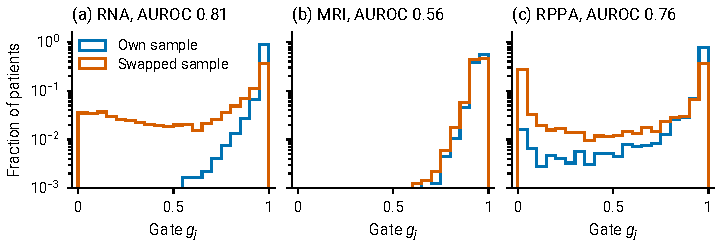
\includegraphics[width=0.72\linewidth]{figures/fig_gate.pdf}
\caption{Verification gate $g_j$ for patients with their own sample (blue) and with a swapped sample (orange), pooled over the internal test folds. The AUROC measures how well the gate separates the two.}
\label{fig:gate}
\end{figure}

\emph{Gate.} Fig.~\ref{fig:gate} shows the gate separates own from swapped samples for RNA (AUROC \GateAucRna{}) and RPPA (\GateAucRppa{}) but not MRI (\GateAucMri{}), whose features barely reflect receptor status. Mean gate values for own samples are \GateTrueRna{} (RNA) and \GateTrueRppa{} (RPPA), so correct contributions are rarely suppressed. For swapped samples, the gate falls below 0.5 in \GateLowRna\% (RNA) and \GateLowRppa\% (RPPA) of cases. Removing CARF's robust term lowers the RNA-swap AUROC to \IntRnaSwapCarfTwoNoRobust{} internally and \ExtRnaSwapCarfTwoNoRobust{} externally (supplementary material). Weak MRI verification reflects a verification-variable problem, not a modeling limit: an exploratory, I-SPY1-only gate built on tumor T-stage (unavailable in I-SPY2, so it cannot fit the main pipeline) separates true from swapped MRI samples far better (AUROC $\MriTstageGateAuc{}$ vs.\ $\GateAucMri{}$; full derivation in the supplement).
\subsection{Anchor failure}
\label{sec:anchor-failure}

CARF bounds displacement from the clinical anchor but cannot protect against a wrong anchor, such as a charting error in HR or HER2 status. Simulating HR/HER2 flips on frozen external models, CARF performs worse than stacking here: at 20\% combined error, the clinical expert reaches \AnchorBothTwoZeroClinical{}, stacking reaches \AnchorBothTwoZeroStack{}, and CARF only \AnchorBothTwoZeroCarf{} ($\DAnchorBothTwoZeroCarfStack{}$), a gap already present at 5\% error. Removing the gate recovers about half of it (\AnchorBothTwoZeroCarfNoGate{}): the gate checks each sample against the same anchor, so it amplifies anchor error rather than tolerating it. This is CARF's most significant limitation: it assumes a correct anchor and should not be deployed where that assumption may fail silently.
\subsection{Naturally missing modalities}
\label{sec:natural}

In I-SPY1, \NatPartialN{} further patients have only expression or MRI; CARF matches the clinical model overall (\NatAllCarfTwo{} vs.\ \NatAllClinical{}) but trails it in the partial subgroup (\NatPartialCarfTwo{} vs.\ \NatPartialClinical{}), so a single optional modality adds no discrimination. On the independent GSE25066 cohort (\GseN{} patients, RNA refit on shared genes), CARF matches the clinical model on intact inputs (\GseIntactCarfTwo{} vs.\ \GseIntactClinical{}) and under RNA swap (\GseRnaSwapCarfTwo{}; full results in the supplement).

\subsection{Budget and robustness trade-off}

Inner cross-validation selects $B\in\{1.5,2\}$ in \BudgetList{} of 25 folds. The unbounded rule is more accurate externally (\ExtCarfTwoUnbounded{}) but less robust (RNA swap \ExtRnaSwapCarfTwoUnbounded{}) and carries no displacement guarantee, unlike CARF's bounded \MaxDispCarfTwo{}-logit maximum, versus up to \MaxDispGatedOffsetLr{} logits for other fusion models (fixed-$B$ and no-swap-training comparisons in the supplement); when every optional modality is removed, CARF returns the clinical prediction exactly.

%======================================================================
\section{Conclusions}

We introduce bounded anchored fusion (CARF), with an anchor-verification gate and a convex objective with sample swaps. On intact inputs it matches unconstrained fusion, guarantees exact fallback and bounded changes, and keeps its margin under two modality failures (supplementary). Platt recalibration corrects most prevalence overestimation (external Brier \CalibExtCarfBrierBefore{}$\to$\CalibExtCarfBrierAfter{}, ECE \CalibExtCarfEceBefore{}$\to$\CalibExtCarfEceAfter{}) without changing ranking. This yields three auditable signals: an exact clinical-only fallback, a thresholdable displacement for review, and a gate that can flag specimen mix-ups. None replaces clinical judgment or QC.

CARF guarantees stability, not accuracy, and is less robust than stacking under an incorrect anchor. Recalibration leaves external ECE above zero and was fit internally. The gate misses within-subtype swaps and barely verifies MRI; an exploratory I-SPY1-only tumor-stage gate does better (AUROC \MriTstageGateAuc{} vs.\ \GateAucMri{}), a direction for future data, not a fix. Mix-ups are simulated, and I-SPY1 informed exploratory screening, so it is not untouched validation. The 112-patient external cohort (31 pCR) is the main limit.

GSE25066 and GSE20194 are RNA-only and 81\% overlapping, so they cannot evaluate MRI, RPPA, or multi-modal failure. No other public cohort pairs MRI, expression, and pCR outcome outside I-SPY1/I-SPY2, so independent multi-modal validation remains infeasible. Future work should test documented mix-ups, tumor-stage cohorts, and a larger independent multi-modal cohort. Code is available at \url{https://github.com/21f2000143/bl2403-carf}.
\bibliographystyle{splncs04}
\bibliography{references}
\end{document}
